\documentclass[t]{beamer}
\setbeamertemplate{navigation symbols}{} %no nav symbols
\usepackage{beamerthemeshadow}
\usepackage{pgf}
\usepackage{listing}
\usepackage{listings}
\usepackage{verbatim}
\usepackage{multirow}
\usetheme{Copenhagen} % Beamer theme v 3.0
\usecolortheme{whale} % Beamer color theme


\usepackage[boxed,linesnumbered,vlined,slide]{algorithm2eCustom}



\title[Fall Presentation 2010\hspace{14em}\insertframenumber/\inserttotalframenumber]{Proactive Caching for Spatial Queries in Mobile Environments \\\&\\ Cache Invalidation and Replacement Strategies for Location-Dependent Data in Mobile Environments}
\author[Jeppe R. Thomsen]{Jeppe R. Thomsen}%\\ \small{jenslyn@cs.aau.dk}}
\institute{Hong Kong Polytechnic University\\ Department of Computing}
\begin{document}
\begin{frame} % Cover slide
\titlepage
\end{frame}
% Instead, you can use \frame{\titlepage}} (Beamer v 2.2 macro)

\section{Introduction} % Bookmark information

\begin{frame}[red]
\frametitle{Overview}
\Large

\end{frame}

\input{cacheInvalid}
\section{Proactive Caching for Spatial Queries in Mobile Environments}

\subsection{Introduction}

\begin{frame}
\frametitle{Introduction}
	\begin{center}
	\Large
	Published at: ICDE '05: Proceedings of the 21st International Conference on Data Engineering\\\vspace{1em}
	by\\\vspace{1em}
	Haibo Hu, Jianliang Xu, Wing Sing Wong, Baihua Zheng, Dik Lun Lee, and Wang-Chien Lee\\\vspace{1em}
	April 2005
	\end{center}
\end{frame}


\begin{frame}
\frametitle{Motivation}
\large


\end{frame}


\begin{frame}
\frametitle{Related Work}
\Large

Caching:
\begin{itemize}\itemsep 16pt
\item Page Caching
\item Semantic Caching
\end{itemize}

\end{frame}

%----------------------------------------------


\subsection{Problem}

\begin{frame}
\frametitle{Problem}

\end{frame}

\begin{frame}
\frametitle{R-Tree}

\begin{center}
\includegraphics[scale=0.95]{images/r-tree.jpg}
\end{center}
\end{frame}

%----------------------------------------------

\subsection{Contribution}

\begin{frame}
\frametitle{Proactive Caching}

\begin{enumerate}
\item Execute query $Q$ on local partial R-tree index and cache
\item If any items are found while executing $Q$ locally, then return immidiately
\item If $Q$ is satisfied then terminate, else Construct $Q_r = Q + H$ and send to server
\end{enumerate}

\begin{center}
\includegraphics[scale=0.55]{images/kNNproactive-caching.jpg}
\end{center}

\end{frame}

\begin{frame}
\frametitle{Proactive Caching}

\begin{center}
\includegraphics[scale=0.80]{images/proactive-caching.jpg}
\end{center}

\end{frame}

\begin{frame}
\frametitle{Response time and Hit rate}

Query responsetime:\\
$resp(Q)=\frac{|R_r|(T{Q_{r}}+\frac{1}{2}|R_r|\cdot T_d}{|R|}$
\vspace{1.5em}

Cache Hit rate:\\
$hit_c = \frac{|R_s|}{R}$
\end{frame}


\begin{frame}
\frametitle{}

Algorithm is a 2-approximation algorithm

When cached node is removed, the children of that item should be considered into the benifit calculations.

$\sum_{j \in D(i)}{prob(j)\times size(i)+ prob(i)\times size(i)}$


\end{frame}


%----------------------------------------------

\subsection{Experimental Results}
%
%\begin{frame}
%\frametitle{Setting}
%\end{frame}
%
%\begin{frame}
%
%\end{frame}
%
%\begin{frame}
%\frametitle{Cache hit ratio / Data Size - scope 1 and 2}
%
%\end{frame}
%
%\begin{frame}
%\frametitle{Cache hit ratio / Query interval - scope 1 and 2}
%
%\end{frame}
%
%\begin{frame}
%\frametitle{Cache hit ratio / Moving interval - scope 1 and 2}
%%\includegraphics[scale=0.5]{images/fig9.jpg}
%
%\end{frame}
%

\begin{frame}
\frametitle{Conclusion}
\Large
Proactive Caching outperforms page caching and semantic caching
\end{frame}

\begin{frame}
\frametitle{Impression}

Their results were not stellar\\

Graphs are "`cut"' just before compeditors might seem to become better

\end{frame}

\section{Tutorial - Fast Fourier Transformation }

\subsection{Introduction}

\begin{frame}
\frametitle{Fast Fourier Transformation}

Speeds up calculations of DFT (Discrete Fourier transform)

Used for fast:
\begin{itemize}
\item Addition of polynomials
\item Multiplication of polynomials
\item Conversion between Coefficient Representation \& Point-value Representation
\end{itemize}
% Interpolate - Evaluate

\includegraphics[scale=0.5]{images/poly-transform.jpg}

\end{frame}

\subsection{Polynomials}

\begin{frame}
\frametitle{Polynomials}
\begin{equation}
A(x) = \sum{^{n-1}_{j=0} \hspace{0.5em} a_jx^i}, \hspace{1.5em} a_j x^3 + a_{j-1} x^2 - a_{j-2} x + 4
\end{equation}


\textbf{Degree:} highest non-zero coefficient 

\textbf{Degree-bound:} Any integer strictly larger than the bound for $A(x)$

\end{frame}


\begin{frame}
\frametitle{Polynomial Addition}

\begin{eqnarray}
A(x) = 6x^3 + 7x^2 - 10x + 9  \\
B(x) = -2x^3 + 4x -5  \\ \hline
C(x) = 4x^3 + 7x^2 - 6x + 4 
\end{eqnarray}


\begin{eqnarray*}
\begin{tabular}{ l r }
 A(x) = & 6x^3 + 7x^2 - 10x + 9  \\
 B(x) = & -2x^3 + 4x -5  \\ \hline
 C(x) = & 4x^3 + 7x^2 - 6x + 4 
 \end{tabular}
\end{eqnarray*}


\end{frame}


\begin{frame}
\frametitle{Polynomial Multiplication}

\begin{itemize}
\item 
\end{itemize}


\end{frame}

\begin{frame}
\frametitle{Fast Fourier Transformation}


\begin{itemize}
\item 
\end{itemize}
% Interpolate - Evaluate



\end{frame}


%\subsection{Problem Setting}

\begin{frame}
\frametitle{Problem Setting}

\begin{columns}
	\begin{column}{0.5\textwidth}
		\only<1>{ 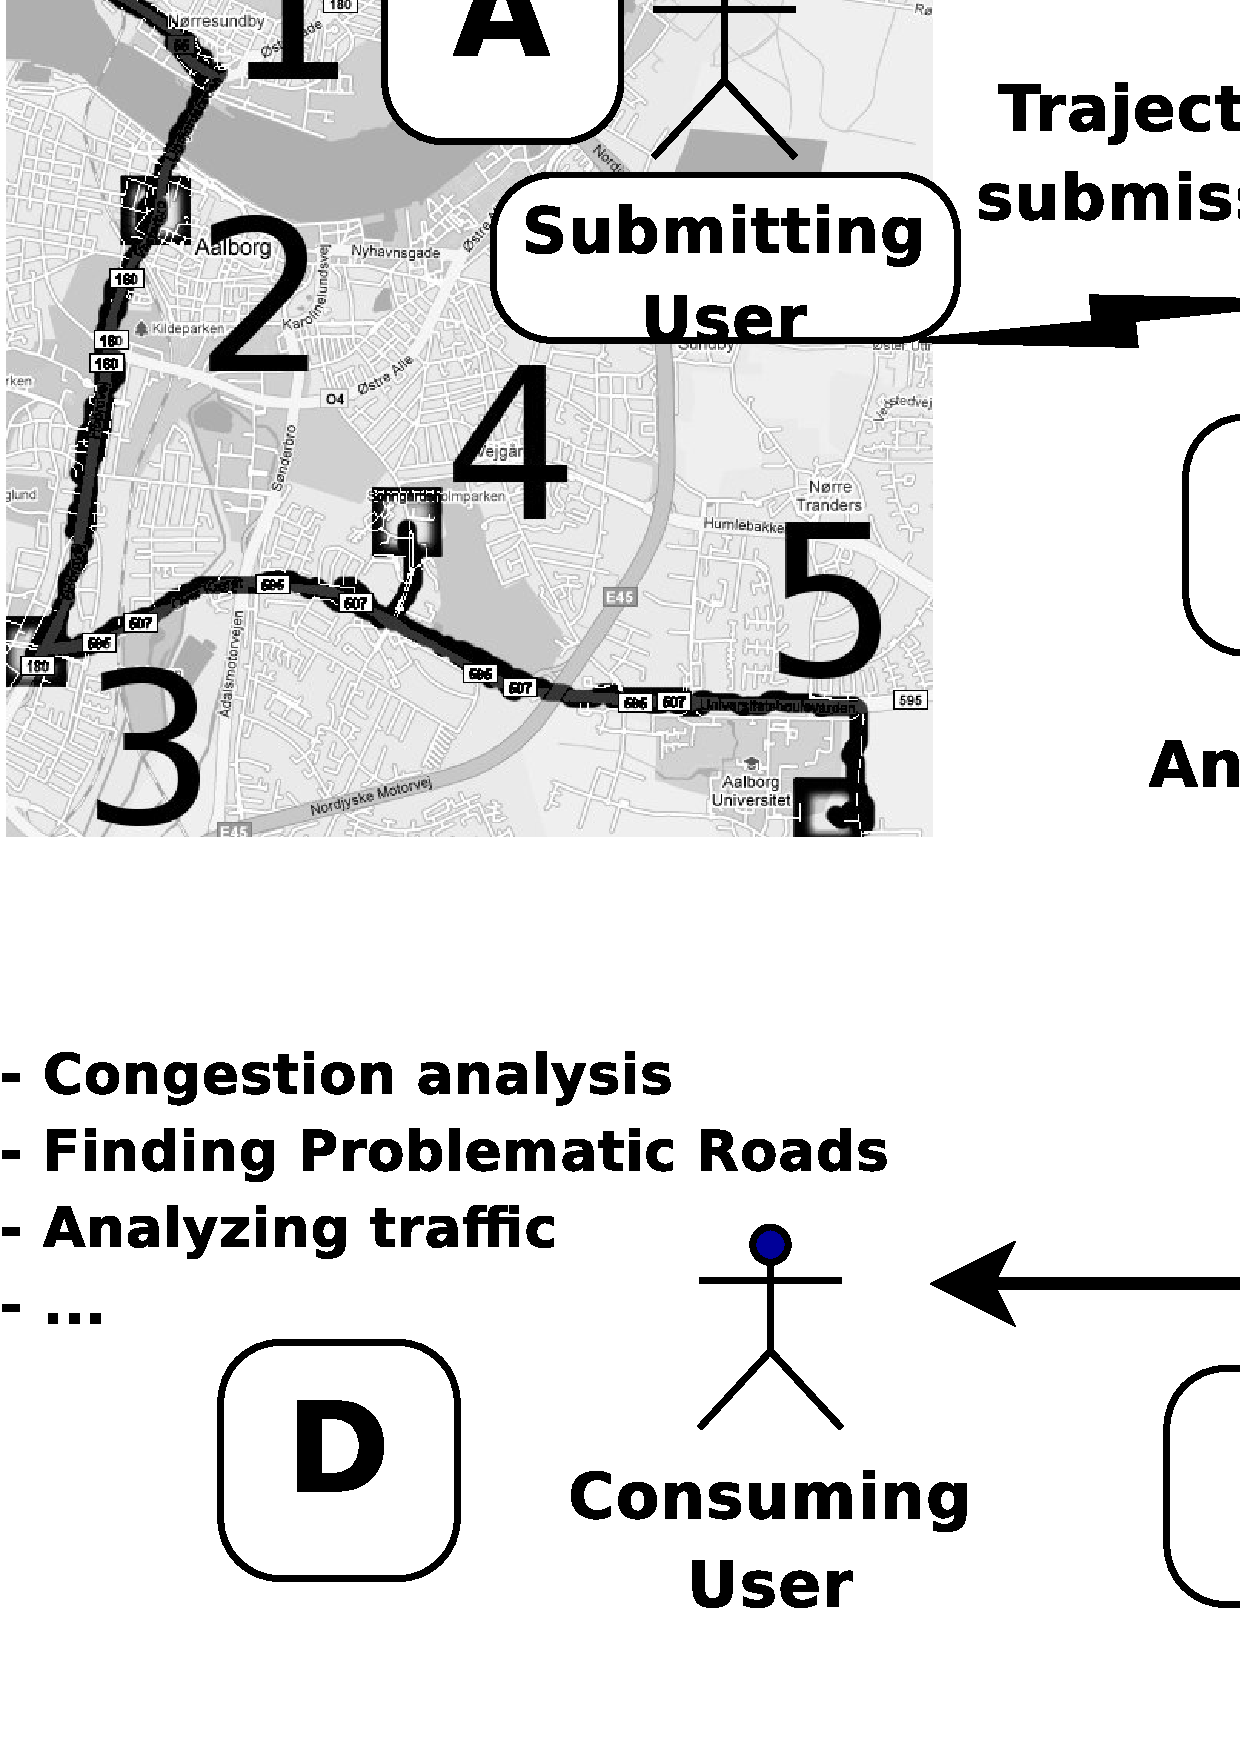
\includegraphics[page=1,scale=0.2]{images/overview.pdf}}
	\end{column}
	\begin{column}{0.5\textwidth}
		\begin{description}\itemsep 16pt
		\item[A] Privacy Aware User
		\item[B] Trusted Server
		\item[C] Public Untrusted Server
		\item[D] Service Providers
		\end{description}
	\end{column}
\end{columns}
\end{frame}
%\subsection{Goals} % Bookmark information, displayed in the progress tree

\begin{frame}[red] %hmm.. thought i could change colour here :S
\frametitle{Goals}

At the service provider:
\begin{itemize}
\item Remove all user identifying information from trajectories.
\item Preserve usability to users of public dataset
\end{itemize}

\vspace{3em}
At the users side:\\

\begin{itemize}
\item  Provide {\bf Usability}. specifying privacy should be simple.
\item Be {\bf Practical}. No user interaction during normal operation.
\item Be {\bf Flexible}. Support several ways of defining privacy.
\end{itemize}

\end{frame}



\subsection{Related work}

\begin{frame}
\frametitle{Related work}

Protection of Trajectories
\begin{itemize}
\item Collapse trajectories and remove updates
\item Only publish edges with k support.
\vspace{1em}
\item At each update compute MBR including k-1 updates
\item Precompute regions before sending.
\vspace{1em}
\item Degrade public dataset so no sub-trajectory can be matched to it.
\end{itemize}
\vspace{1em}
{\Large \bf No work on spatial anonymity with time}
\end{frame}
%\section{Privacy Profile}

\begin{frame}[red]
\frametitle{Privacy Profile}
\begin{itemize}
\item Settings
\item PSR - Potentially Sensitive Region
\item Protection types and schemes
\item t-anonymity
\end{itemize}
\end{frame}

\subsection{Settings} % Bookmark information, displayed in the progress tree

\begin{frame}[red] %hmm.. thought i could change colour here :S
\frametitle{Settings}

Users Can
\begin{itemize}
	\item Set both globally and locally
	\begin{itemize}
		\item Temporal sensitivity
		\item Spatial sensitivity
	\end{itemize}
	\item Define a PSR
	\item Have multiple profiles.
\end{itemize}

\vspace{1em}
\begin{definition}[Privacy Profile]
$\left(stime,etime,d_s, d_t,\{PSR \} \right)$
\end{definition}

\end{frame}



\begin{frame}[red] %hmm.. thought i could change colour here :S
\frametitle{PSR}
\begin{itemize}
\item A group of edges in a road network considered sensitive
\item A value indicating spatial sensitivity
\item A value indicating temporal sensitivity
\item A general usage class
\end{itemize}
\begin{definition}[PSR]
A PSR $p$ is a tuple $(p_{edges}, d_s, d_t, class)$ where $p_{edges}$ is the set of tuples $\{(e, e_{from}, e_{to} | 0 \leq e_{from} < e_{to} \leq e_{length})\}$ which is sensitive. 
$e \in \mathbf{E}$ and $e_{from}, e_{to}, e_{length} \in \mathbb{R}$. 
$e_{from}/e_{to}$ specifies on $e$ the start-/end-location covered by $p_{cover}$. If $e$ is fully included in $p_{cover}$, $e_{from}/e_{to}$ is equal to $0/p_{length}$.
$d_s, d_t, class \in \mathbb{N}$ is respectively the spatial sensitivity, the temporal sensitivity, and the PSR classification
\end{definition}
\end{frame}

\begin{frame}[red] %hmm.. thought i could change colour here :S
\frametitle{PSR Classes}

\begin{table}
%\begin{tabular*}{0.8\columnwidth}{|p{0.2\columnwidth}|l|p{0.25\columnwidth}|}
\begin{tabular}{|l|l|}
\hline
\bf Classification	& \bf Scheme \\\hline		
Public Service Point	& AS \\\hline
House			& ASTI,RS \\\hline
Route w. endpoints	& AS, ASTI, RS  \\\hline
Route w/o endpoints	& AS, ASTI, RS  \\\hline
\end{tabular}
\end{table}
\vspace{1em}

Protection Schemes
\begin{itemize}
	\item AS - Always Sensitive.
	\item ASTI - Always Sensitive within a time interval.
	\item RS - Rarely Sensitive.
\end{itemize}
\end{frame}


\subsection{t-anonymity} 
\begin{frame}[red]
\frametitle{t-anonymity}

Spatial k-anonymity 
\begin{itemize}
\item Adapted for trajectories
\item Argumented with time.
\end{itemize}
\vspace{1em}

In a PSR:
\begin{itemize}
\item Spatial sensitivity decides t-1 trajectories to hide between
% \vspace{1em}
\item Temporal sensitivity defines a time period shared with t-1 other trajectories.
\end{itemize}
\end{frame}


\begin{frame}[red] %hmm.. thought i could change colour here :S
\frametitle{Definition: t-anonymity}
\begin{definition}[t-anonymity]
Given $\mathbf{T}$, the set of trajectories and $p_{edges}$, the set of edges covering a sensitive part of trajectory $\gamma$. 

Let $\Gamma \subseteq \mathbf{T}$ be all trajectories which subtrajectories intersect with $p_{edges}$. $\Gamma' \subseteq \Gamma$ be all trajectories where, for edges intersecting with $p_{edges}$, at each timestamp of $\gamma$ their timestamps lie within a time period $TP$ symmetric around the timestamp of $\gamma$.

$\Gamma'$ is said to satisfy t-anonymity with respect to $TP$ and $\gamma$ iff $\Gamma'$ contains at least $t-1$ other trajectories.
\end{definition}
\end{frame}

\subsection{Time Period}
\begin{frame}[red]
\frametitle{Time Period}
\begin{columns}
	\begin{column}{0.5\textwidth}
		\only<1>{ 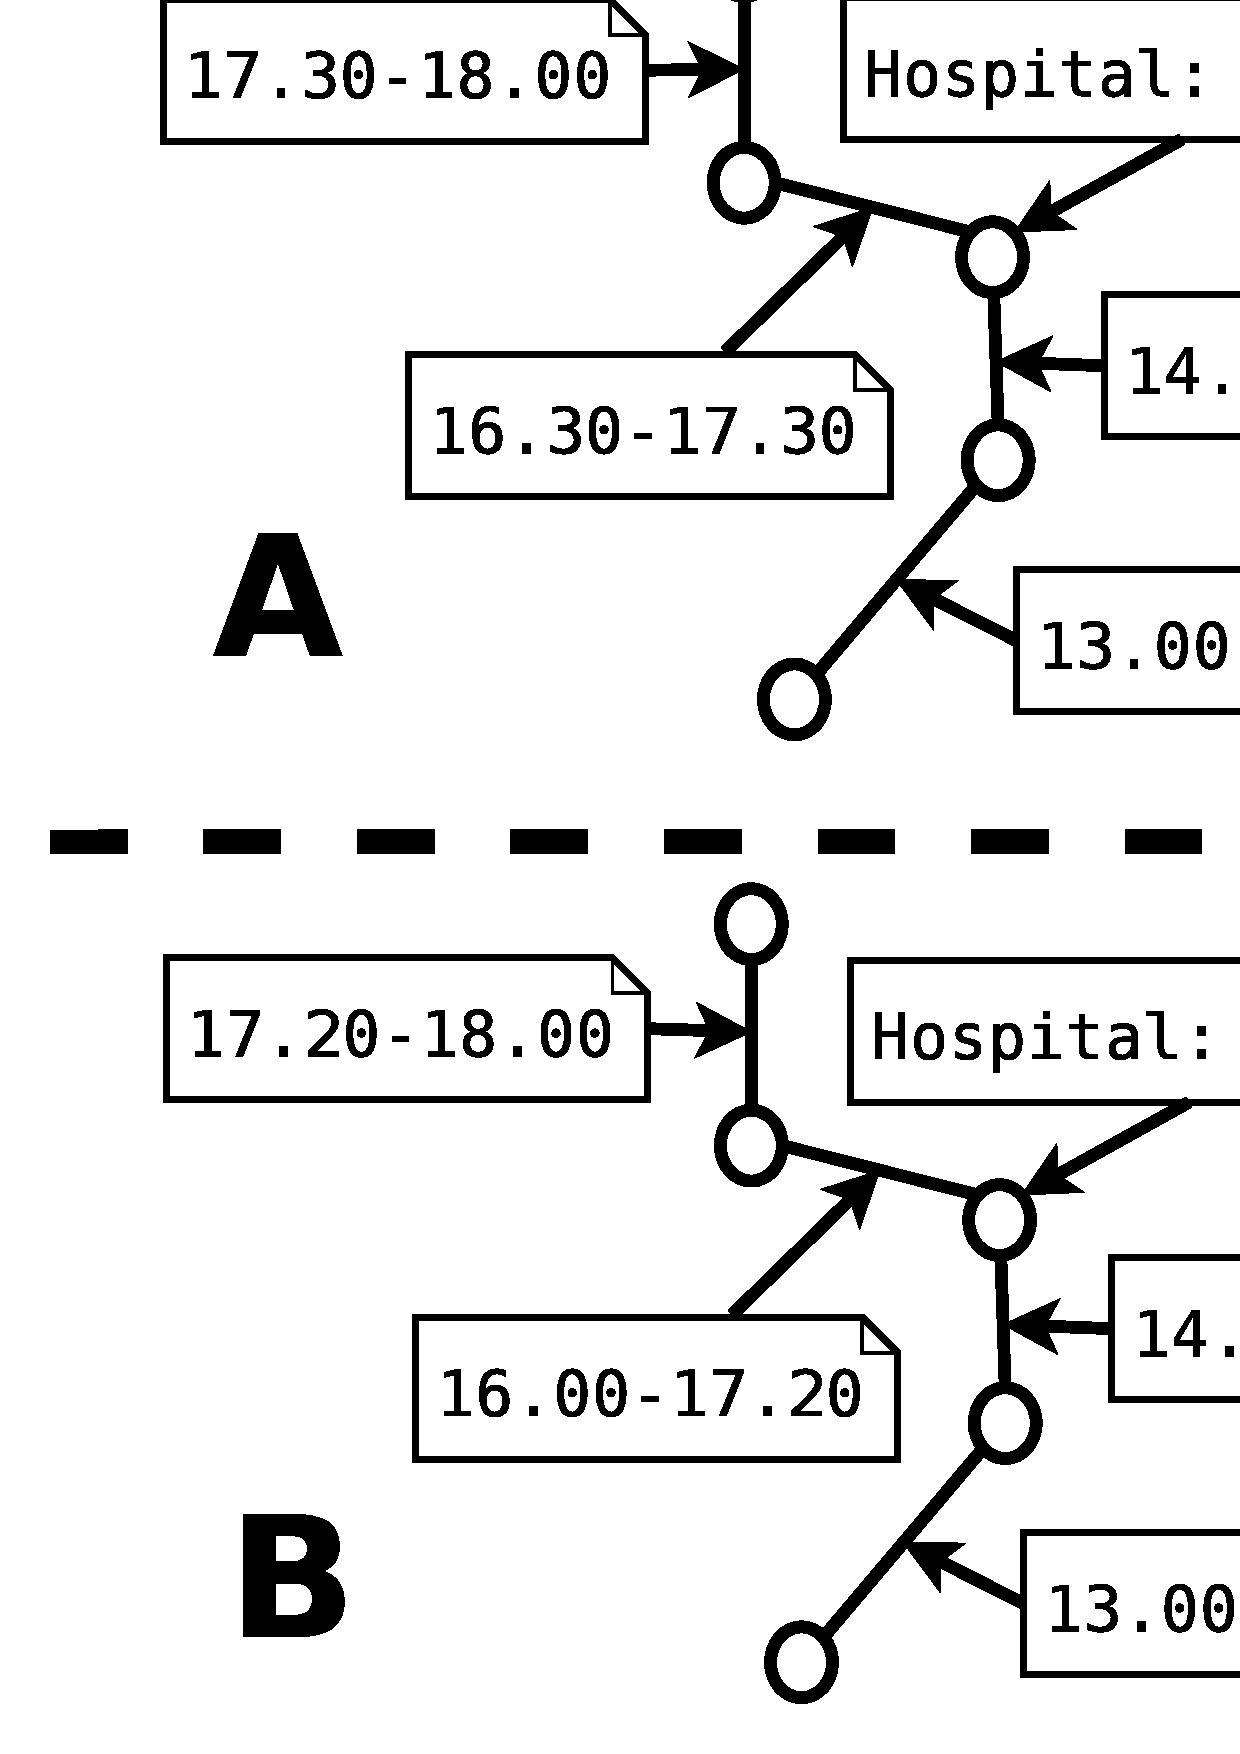
\includegraphics[scale=0.16]{images/trajecAdjustTime.pdf}}
	\end{column}
	\begin{column}{0.5\textwidth}
		\only<1>{ \includegraphics[scale=0.8]{images/trajecAdjustTimeGraph.pdf}}
	\end{column}
\end{columns}
\end{frame}
%\section{Conclusion}
\subsection{Conclusion} % Bookmark information, displayed in the progress tree
\begin{frame}[red] %hmm.. thought i could change colour here :S
\frametitle{Conclusion}

\begin{itemize}
	\item Novel Privacy Profile to specify spatial-temporal sensitivity of a POI.
	\item Introduced t-anonymity
	\item Introduced Protection types and schemes.

\end{itemize}

 
\end{frame}

\subsection{Future Work} % Bookmark information, displayed in the progress tree
\begin{frame}[red] %hmm.. thought i could change colour here :S
\frametitle{Future Work}

\begin{itemize}
	\item Algorithm
	\item Performance study

\end{itemize}
\end{frame}


\begin{frame}[red] %hmm.. thought i could change colour here :S
\frametitle{End of Presentation}

\vspace{20mm}
\begin{center}
    \Huge Thank You For Listening
\end{center}

\end{frame}

\end{document}

%General
%
%    * Is it clear where the paper was published and by whom?
%    * Does the talk have a concrete motivating example very early?
%    * Are unfamiliar abbreviations introduced and used appropriately?
%    * Is the main problem addressed in the paper clearly stated?
%    * Does the presentation have concrete and minimal examples of core ideas?
%    * Are dynamics, e.g., searching a tree presented using animation techniques?
%    * Are the listeners background use appropriately, e.g., no need to tell what an array is, however must tell what the XY++-Tree is?
%    * Is there a reasonable number of slides in total in the presentation?
%
%Figures
%
%    * Are complicated figures presented in sufficient details?
%    * Are the symbols used in the figures clear to the listeners?
%
%Performance Graphs
%
%    * Is data, queries, modification, and transactions appropriately introduced?
%    * Are the axis on performance graphs clearly explained?
%    * Are the main conclusion from the graph clearly stated?
%    * Is there only one graph per slide (or are graphs compared)?
%
%Critique
%
%    * Is the critique relevant and fair?
%    * Is the critique balanced?
%    * Is the critique points concrete, i.e., not "it is a good paper"?
